\chapter{Dummy}

\begin{figure}[htbp!]
\caption{Náhodný výběr z~rozdělení $\mathcal{N}_2(\boldsymbol{0},\,I)$}
\label{obr03:Nvyber}
\begin{center}
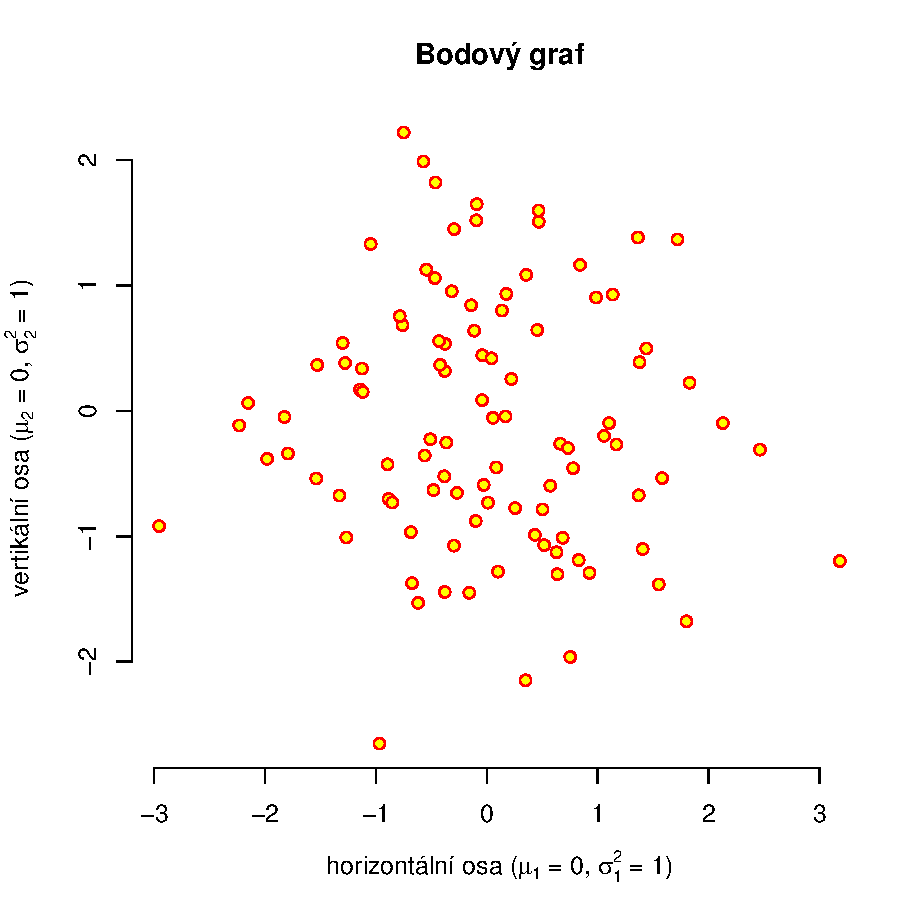
\includegraphics[width=.525\textwidth]{img/ukazka-obr01}
% Příponu není potřeba explicitně uvádět, pdflatex automaticky hledá pdf.
% Rozměry také není nutné uvádět.
\end{center}

\footnotesize \textit{Poznámka:} 
Vlastní zpracování na základě dat z ČSÚ.
\end{figure}

\begin{table}[htbp!]

\begin{center}
%%% Tabulka používá následující balíčky:
%%%   - booktabs (\toprule, \midrule, \bottomrule)
%%%   - dcolumn (typ sloupce D: vycentrovaná čísla zarovnaná na
%%%     desetinnou čárku
%%%     Všimněte si, že ve zdrojovém kódu jsou desetinné tečky, ale
%%%     tisknou se čárky.

\caption{Maximálně věrohodné odhady modelů 1 a 2}\label{tab03:Nejaka}
\begin{tabular}{lrr}
\toprule
              & \multicolumn{1}{c}{\textbf{1}} & \multicolumn{1}{c}{\textbf{2}}\\
\midrule
\multirow{2}{*}{Abs. člen}     &$-10,01$***  &42,01**\\
                               & (1,01)      &(1,89)\\
\multirow{2}{*}{Pohlaví (muž)} &	9,89*       & 8,16\\
                               & (5,98)	    &(8,18)\\
Výška (cm)                	   & 0,78***     &(0,12)	\\
\bottomrule
\end{tabular}
\end{center}

\footnotesize \textit{Poznámka:} 
(i) V závorkách jsou uvedeny směrodatné chyby získané na základě 500 iterací neparametrického bootstrapu.\\
(ii) * p < 0,05, ** p < 0,01, *** p < 0,001.\\
(iii) Vlastní zpracování na základě dat z ČSÚ.
\end{table}

\begin{code}{Python}{Ukázka zpracování pomocí Pythonu}{zpracovani-python}
import numpy as np
    
def incmatrix(genl1,genl2):
    m = len(genl1)
    n = len(genl2)
    M = None #to become the incidence matrix
    VT = np.zeros((n*m,1), int)  #dummy variable
    
    #compute the bitwise xor matrix
    M1 = bitxormatrix(genl1)
    M2 = np.triu(bitxormatrix(genl2),1) 

    for i in range(m-1):
        for j in range(i+1, m):
            [r,c] = np.where(M2 == M1[i,j])
            for k in range(len(r)):
                VT[(i)*n + r[k]] = 1;
                VT[(i)*n + c[k]] = 1;
                VT[(j)*n + r[k]] = 1;
                VT[(j)*n + c[k]] = 1;
                
                if M is None:
                    M = np.copy(VT)
                else:
                    M = np.concatenate((M, VT), 1)
                
                VT = np.zeros((n*m,1), int)
    
    return M
\end{code}
